\section{Detailed Mechanistic View of Augmentation Strategies}
\label{app:detailed_augmentation_diagrams}

This appendix section provides a more granular, node-based representation (Figure~\ref{fig:detailed_augmentation_node_graph_appendix}) to elaborate on the hypothesized attribute interactions and the counterfactual generation process. This detailed view aims to offer a causal understanding that complements the main paper.

Figure~\ref{fig:detailed_augmentation_node_graph_appendix} aims to provide a deeper, causal understanding of the causal perturbation process through which we obtain our causal upgradations and degradations. We term the spurious attributes that move when causal attributes are intervened upon as $SP_2(A) \subset SP(A)$ for any answer $A$.

\paragraph{Part 1: Causal Augmentation (Attribute Upgradation/Degradation).}
We first generate a counterfactual Answer 2 from an original Answer 1 (for query $\mathrm{Q}$) via an LLM-driven "Counterfactual Generation Process." This process intervenes to modify a specific causal attribute $C_j$ within Answer 1's causal profile $\mathrm{C(A1)}$ to a target state $C'$, resulting in $\mathrm{C(A2)}$. 
We aim to keep spurious attributes fixed by asking for a minimal perturbation. Therefore attributes $\mathrm{SP_1(A1)}$ are ideally preserved.
% While spurious attributes $\mathrm{SP_1(A1)}$ are ideally preserved, 
Yet, $\mathrm{SP_2(A1)}$ (which may co-vary with $\mathrm{C(A1)}$) might transition to $\mathrm{SP_2(A2)}\neq\mathrm{SP_2(A1)}$. The goals of this transformation are to ensure $A_2$ reflects the intended causal change. The RM is then trained on the pair $(A_1, A_2)$ with a preference label reflecting the upgrade/degradation, teaching sensitivity to isolated causal attribute modifications. 

\paragraph{Part 2: Neutral Augmentation (via Irrelevant Query).}
As illustrated in Figure \ref{fig:detailed_augmentation_node_graph_appendix}, we need spurious invariance to $SP_2$ which are hard to disentangle as well. This illustrates the need for an intervention free method for neutral augmentation like IQN. When we present an answer pair ($A_1, A_2$) from $\mathcal{D}_{\mathrm{pref}} \cup \mathcal{D}_{\mathrm{causal}}$,
re-contextualized with a new, unrelated query $\mathrm{Q}_{\text{irrelevant}}$,
we teach the model invariance to $(SP_1, SP_2)$.
This is because, the primary differences between $A_1$ and $A_2$ in this new context are their spurious attributes ($\mathrm{SP_1}$,$\mathrm{SP_2}$). 
Note that the causal difference between $A_1$ and $A_2$ in $\mathcal{D}_{\mathrm{pref}} \cup \mathcal{D}_{\mathrm{causal}}$ in presence of irrelevant query is now spurious, and hence there need not be any sensitivity to it.


\begin{figure}[!t]
    \centering
    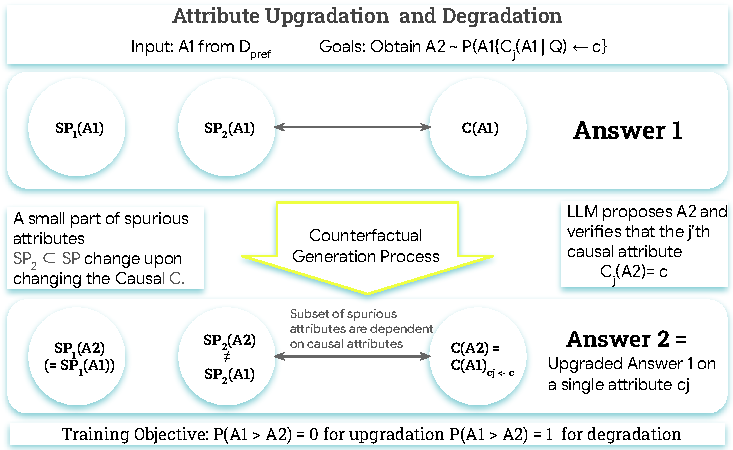
\includegraphics[width=0.9\linewidth]{images/CausalAugmentationGraph.pdf}
    \caption{Detailed mechanistic diagram of \carma's Causal Attribute Upgradation and Degradation, illustrating attribute components and transformations. This causal diagram indicates that on changing causals some spurious features also can get dragged along (we call these $SP_2$). Hence separating these is very hard. This illustrates the need for a neutral augmentation strategy that provides invariance to $SP_2$ attributes.}
    \label{fig:detailed_augmentation_node_graph_appendix}
\end{figure}

